%/* vim: set filetype=latex */

% Demo project. Uses Komascript >=3.0. 
% which is not included in texlive 2008
% (1) copy dist to texlive/texmf-local 
% (2) texhash
%\documentclass[BCOR=8.5mm,DIV=calc,open=right,pagesize=auto,a5paper]{scrbook}
%\documentclass[12pt,BCOR=8.5mm]{scrbook}
\documentclass[11pt,BCOR=8.5mm]{scrartcl}

% Use utf-8 encoding for foreign characters
\usepackage[utf8]{inputenc}
\title{Amateurfunkprüfung}
\subtitle{Prüfungsteil "`Betriebstechnik und Vorschriften"'}
\author{Mathias Dalheimer \texttt{<md@gonium.net>}}
%% PDF SETUP
\usepackage[pdftex, bookmarks, colorlinks, breaklinks,
pdftitle=\title,pdfauthor={Mathias Dalheimer},plainpages=false]{hyperref}  
\hypersetup{linkcolor=blue,citecolor=blue,filecolor=black,urlcolor=blue,plainpages=false} 

\clubpenalty=3000 % adjust for widows and orphans 10000 is max
\widowpenalty=3000 % adjust for widows and orphans 10000 is max
%% Font Adjustments
\usepackage[LY1]{fontenc}
\usepackage[T1]{fontenc}
%\usepackage{adobegaramond}
%\usepackage{gillsans}
%\renewcommand{\rmdefault}{HoeflerText}

% Use URW Garamond No. 8 as a default font. (getnonfreefonts)
%\usepackage[urw-garamond]{mathdesign}
%\renewcommand{\rmdefault}{ugm}
% Optima as a sans serif font.
%\renewcommand*\sfdefault{uop}

\newcommand*\imgwidth{0.8\textwidth}
\usepackage{longtable}
\usepackage{ifthen}
\newboolean{InternalVersion}
\setboolean{InternalVersion}{true}
%\setboolean{InternalVersion}{false}

\usepackage{listings}  
\lstset{numbers=left, numberstyle=\tiny,numbersep=5pt}  
\lstset{language=Xml, basicstyle=\small, frame=shadowbox}  

\usepackage{algorithmic}
\usepackage{algorithm}
%\numberwithin{algorithm}{chapter} 
%\newcommand{\theHalgorithm}{\arabic{algorithm}}

\usepackage[protrusion=true,expansion=true]{microtype}

%% Page Header
\usepackage{scrpage2}

% Recalculate page setup based on new font.
%\KOMAoptions{DIV=last}
%\KOMAoptions{draft=true}

% Versals. 
%\usepackage{lettrine}
% Misc packages
\usepackage{url}
\usepackage{graphicx}
\usepackage{todonotes}
%\usepackage[english]{babel}
\usepackage{ngerman}
\usepackage{blindtext}
\usepackage{subfigure}

\hyphenation{scho-oner Sur-vivor ap-pen-dix
Strom-ver-brauchs-informationen}

\usepackage{marvosym} % bei der Schrift enthalten
\newcommand*\euro{\textup{\EUR}}


%% Chapterstyle
%\renewcommand*{\chapterformat}{---\hskip.5cm\thechapter\hskip.5cm---}
%\KOMAoption{headings}{small,twolinechapter}
%\setkomafont{chapter}{\Large\sffamily\centering}
%\setkomafont{dictum}{\normalfont}
%\renewcommand*{\dictumwidth}{.8\textwidth}

%% Main.
\begin{document}
\maketitle
%\clearscrheadfoot
%\automark[chapter]{section}
%\lehead[]{\pagemark\hskip.5cm\vrule\hskip.5cm\title}
%\rohead[]{\headmark\hskip.5cm\vrule\hskip.5cm\pagemark} 
\title
%\pagestyle{scrplain}
%\begin{titlepage}
%\input{frontpage}
%\end{titlepage}
%% frontmatter
%%\input{frontmatter}
%%\parindent.0cm
%%\parskip.4cm
%%\input{pagetwo}
%\parindent.4cm
%\parskip.0cm
%\pagestyle{scrheadings}
%
\section{Internationales Buchstabieralphabet}

\begin{table}[h]
  \centering
\begin{tabular}[h]{|l|l|}
  \hline
  Buchstabe & Schlüsselwort \\
  \hline
  \hline
  A & Alpha \\
  B & Bravo \\
  C & Charlie \\
  D & Delta \\
  E & Echo \\
  F & Foxtrott \\
  G & Golf \\
  H & Hotel \\
  I & India \\
  J & Juliett \\
  K & Kilo \\
  L & Lima \\
  M & Mike \\
  N & November \\
  O & Oscar \\
  P & Papa \\
  Q & Quebec \\
  R & Romeo \\
  S & Sierra \\
  T & Tango \\
  U & Uniform \\
  V & Victor \\
  W & Whiskey \\
  X & X-Ray \\
  Y & Yankee \\
  Z & Zulu \\
  \hline
\end{tabular}
\end{table}

\section{Der Q-Schlüssel}

Alle Zeiten in UTC! Nur im Telegrafiefunkverkehr verwenden! Skala 1-5: 1
entspricht wenig, 5 entspricht viel.

\begin{table}[h]
  \centering
  \begin{tabular}{| l | p{4.3cm} | p{4.3cm} | l |}
  \hline
  Q-Code & ! & ? & Merke \\
  \hline
  \hline
  QRK & Die Verständlichkeit ihrer Zeichen ist (1-5) & Wie ist die
  Verständlichkeit meiner Zeichen? & Verständlichkeit \\
  \hline
  QRM & Ich werde gestört (1-5) & Werden Sie gestört? & Matsch \\
  \hline
  QRN & Ich werde durch atmosphärische Störungen beeinträchtigt (1-5) &
  Werden sie durch atmosphärische Störungen beeinträchtigt? &
  Noise \\
  \hline
  QRO & Erhöhen Sie die Sendeleistung & Soll ich die
  Sendeleistung erhöhen? & Output \\
  \hline
  QRP & Verringern Sie die Sendeleistung & Soll ich die
  Sendeleistung vermindern? & Pipi \\
  \hline
  QRT & Stellen Sie die Übermittlung ein. & Soll ich die
  Übermittlung einstellen? & Terminate \\
  \hline
  QRV & Ich bin bereit & Sind Sie bereit? & Bin bereit \\
  \hline
  QRX & Ich werde Sie um \ldots Uhr wieder rufen. & Wann werden
  Sie mich wieder rufen? & Pause \\
  \hline
  QRZ & Sie werden von \ldots gerufen & Von wem werde ich
  gerufen? & Wer ruft? \\
  \hline
  QSB & Die Stärke Ihrer Zeichen schwankt. & Schwankt die Stärke
  meiner Zeichen? & Bold \\
  \hline
  QSL & Ich gebe Ihnen Empfangsbestätigung. & Können Sie mir
  Empfangsbestätigung geben? & \\
  \hline
  QSO & Ich kann mit \ldots unmittelbar verkehren. & Können Sie
  mit \ldots verkehren? & \\
  \hline
  QSY & Gehen Sie auf eine andere Frequenz über & Soll ich auf
  eine andere Frequenz übergehen? & \\
  \hline
  QTH & Mein Standort ist \ldots Breite, \ldots Länge & Welches
  ist Ihr Standort? & Home \\
  \hline
\end{tabular}
\end{table}

\section{Betriebliche Abkürzungen}
Aus dieser Sektion werden nur recht wenige \$Dinge abgefragt --- zu
einem späteren Zeitpunkt nochmal auf Vollständigkeit prüfen. Interessant
ist auf jeden Fall der Ausschnitt aus einer Telegrafie-Kommunikation auf
Seite 20.

"`Durch die Verwendung von Betriebsabkürzungen und Q-Gruppen wird der
Betriebsablauf vereinfacht und der übertragene Informationsgehalt pro
Zeiteinheit optimiert."'

\begin{table}[h]
  \centering
  \begin{tabular}{| l | l | }
  \hline
  Abkürzung & Bedeutung \\
  \hline
  \hline
  CW & Morse-Telegrafie (Continuous Wave) \\
  \hline
  CQ & Allgemeiner Anruf \\
  \hline
  DE & Deutsche Empfangsstation \\
  \hline
  DX & Distance: KW $\rightarrow$ interkontinental, UKW $\rightarrow$ 
	  300 km \\
  \hline
  OM & Old Man (Funker) \\
  \hline
  OP & Operator (Funker an Klubanlage) \\
  \hline
  YL & Young Lady (Funkerin) \\
  \hline
  PSE & Please \\
  \hline
  VY & very \\
  \hline
  73 & Best Regards \\
  \hline
  WX & Wetter \\
  \hline
  TX & Transmitter (Sender) \\
  \hline
  RX & Receiver (Empfänger) \\
  \hline
  R & Am Anfang einer Antwort: "`Received"' \\
  \hline
  K & Aufforderung zum Senden (oKay) \\
  \hline
  BK & Signal zu Unterbrechung der Sendung (BreaK) \\
  \hline
\end{tabular}
\end{table}
 

\section{Gesetze, Vorschriften und Regelungen}
\subsection{Radio Regulations (RR)}
RR sind in Deutschland durch die "`Vollzugsordnung für den Funkdienst"'
(VO Funk) umgesetzt. Die RR gelten für \emph{alle} Funkdienste.  
RR definiert den \emph{Amateurfunkdienst} und den \emph{Funkamateur}:
\begin{quote}
  "`Der \emph{Amateurfunkdienst} dient zur eigenen Ausbildung, für den
  Funkverkehr der Funkamateure untereinander und für technische
  Studien."'
\end{quote}

\begin{quote}
  "`\emph{Funkamateure} sind ordnungsgemäß ermächtigte Personen, die sich mit
  der Funktechnik aus rein persönlicher Neigung und nicht aus geldlichem
  Interesse beschäftigen."'
\end{quote}

Die RR betrachtet sowohl terestrischen als auch satellitengebundenen
Funkverkehr, fasst das beim Amateurfunk allerdings zusammen.

\subsection{Amateurfunkgesetz (AFuG)}\label{sub:amateurfunkgesetz}
Das AFuG bildet die Rechtsgrundlage für Amateurfunk in Deutschland und
setzt die RR in nationales Recht um. Es regelt die
\emph{Voraussetzungen} und \emph{Bedingungen} für die Teilnahme am
Amateurfunk. Die Bundesnetzagentur (BNetzA) nimmt in Deutschland diese
Aufgaben wahr.

Ziel des Amateurfunkdiensts nach dem AFuG:
\begin{quote}
  "`Zur Ausübung des Amateurfunks aus persönlicher Neigung und nicht aus
  gewerblich-wirtschaftlichem Interesse."'
\end{quote}

\subsection{Amateurfunkverordnung (AFuV)}\label{sub:amateurfunkverordnung}
Regelt die Feinheiten des Amateurfunks im Rahmen des AFuG.
Prüfungsrelevant sind 3 Definitionen:
\begin{enumerate}
  \item Eine "`\emph{Klubstation}"' ist eine Amateurfunkstelle, die von
	Mitgliedern einer Gruppe von Funkamateuren unter Verwendung eines
	gemeinschaftlich genutzten Rufzeichens betrieben wird.
  \item Eine "`\emph{fernbediente oder automatisch arbeitende
	Amateurfunkstelle}"' ist eine unbesetzt betriebene Amaterufunkstelle,
	die fernbedient oder selbsttätig Aussendungen erzeugt
	(Relaisfunkstellen, Digipeater, Funkbaken).
  \item Die "`\emph{Spitzenleistung (PEP)}"' ist die Leistung, die der
	Sender unter normalen Betriebsbedingungen während einer Periode der
	Hochfrequenzschwingung bei der höchsten Spitze der
	Modulationshüllkurve durchschnittlich an einen reellen
	Abschlusswiderstand abgeben kann.
\end{enumerate}

\subsection{Telekommunikationsgesetz (TKG)}\label{sub:telekommunikationsgesetz}
 Einige Regelungen sind auch für den
Amateurfunkdienst anwendbar.
\begin{enumerate}
  \item \emph{Fernmeldegeheimnis:} Empfang von Nachrichten, die nicht für
	Funkamateure, die Allgemeinheit oder einen unbestimmten
	Personenkreis bestimmt sind. Wenns passiert: Keine
	Weitergabe/Nutzung.
  \item \emph{Genehmigung von Sendefunkanlagen:} Jede
	Fernmeldeeinrichtung, die Grundstücksgrenzen überschreitet, ist
	genehmigungspflichtig. Sendefunkanlagen bedürfen ausnahmslos einer
	Frequenzzuteilung, unabhängig von Sendeleistung und Frequenz.
	Nutzung ohne Zuteilung ist eine Ordnungswidrigkeit.
  \item \emph{Wanzen:} Verboten ist Besitz und Betrieb von Sendeanlagen, die einen
	anderen Gegenstand vortäuschen und zum Abhören des nicht öffentlich
	gesprochenen Wortes geeignet sind.
\end{enumerate}

\subsection{Gesetz über Funkanlagen und
TK-Endeinrichtungen (FTEG)}\label{sub:elekommunikationsendeinrichtungen}
Vorschriften für Geräte (Handel/Inbetriebnahme).
\begin{enumerate}
  \item Seriengefertigte Geräte (Empfangsfunkanlagen) müssen FTEG (\& CE) entsprechen.
  \item Wird nicht angewendet bei Amateurfunkgeräten, die nicht im
	Handel erhältlich sind.
  \item Für selbst gebaute Amateurfunkgeräte wird kein Nachweis der
	Einhaltung technischer Vorschriften, da der Amateurfunkdienst ein
	Experimenierfunkdienst ist.
\end{enumerate}

\section{Landeskenner}\label{sec:landeskenner}
%\begin{table}[h]
  \begin{longtable}{| l | l | l |}
  \hline
  Kenner & Land & Hint \\
  \hline
  \hline
  \endhead
  C3 & Andorra & \\
  \hline
  CT & Portugal & \\
  \hline
  DL & Deutschland (DA-DR) & \\
  \hline
  EA & Spanien & EspanA\\
  \hline
  EI & Irland & Eire \\
  \hline
  EM & Ukraine & \\
  \hline
  ES & Estland & \\
  \hline
  F & Frankreich & \\
  \hline
  G & England / Großbritanien & \\
  \hline
  GM & Schottland & \\
  \hline
  HA & Ungarn & \\
  \hline
  HB & Schweiz & \\
  \hline
  HB0 & Lichtenstein & Bei der Schweiz \\
  \hline
  HV & Vatikan & Heiliger Vater \\
  \hline
  I & Italien & \\
  \hline
  LA & Norwegen & Lachse \\
  \hline
  LX & Luxemburg & \\
  \hline
  LY & Litauen & \\
  \hline
  LZ & Bulgarien & \\
  \hline
  M & England, Großbritanien & \\
  \hline
  OE & Österreich & \\
  \hline
  OH & Finnland & \\
  \hline
  OK & Tschechien & \\
  \hline
  OM & Slowakei & \\
  \hline
  ON & Belgien & \\
  \hline
  OY & Färöer Inseln & \\
  \hline
  OZ & Dänemark & \\
  \hline
  PA & Niederlande & \\
  \hline
  UA & Russland & \\
  \hline
  SM & Schweden & \\
  \hline
  SP & Polen & \\
  \hline
  SV & Griechenland & \\
  \hline
  S5 & Slovenien & \\
  \hline
  TA & Türkei & \\
  \hline
  TF & Island & \\
  \hline
  YL & Lettland & \\
  \hline
  YO & Rumänien & \\
  \hline
  YU & Serbien & \\
  \hline
  Z3 & Albanien & \\
  \hline
  3A & Monaco & \\
  \hline
  4U & Vereinte Nationen & For you \\
  \hline
  9A & Kroatien & \\
  \hline
  9H & Malta & \\
  \hline
\end{longtable}

\subsection{Europakenner in der Karte}\label{sub:europakarte}

\begin{figure}[htbp]
  \begin{center}
	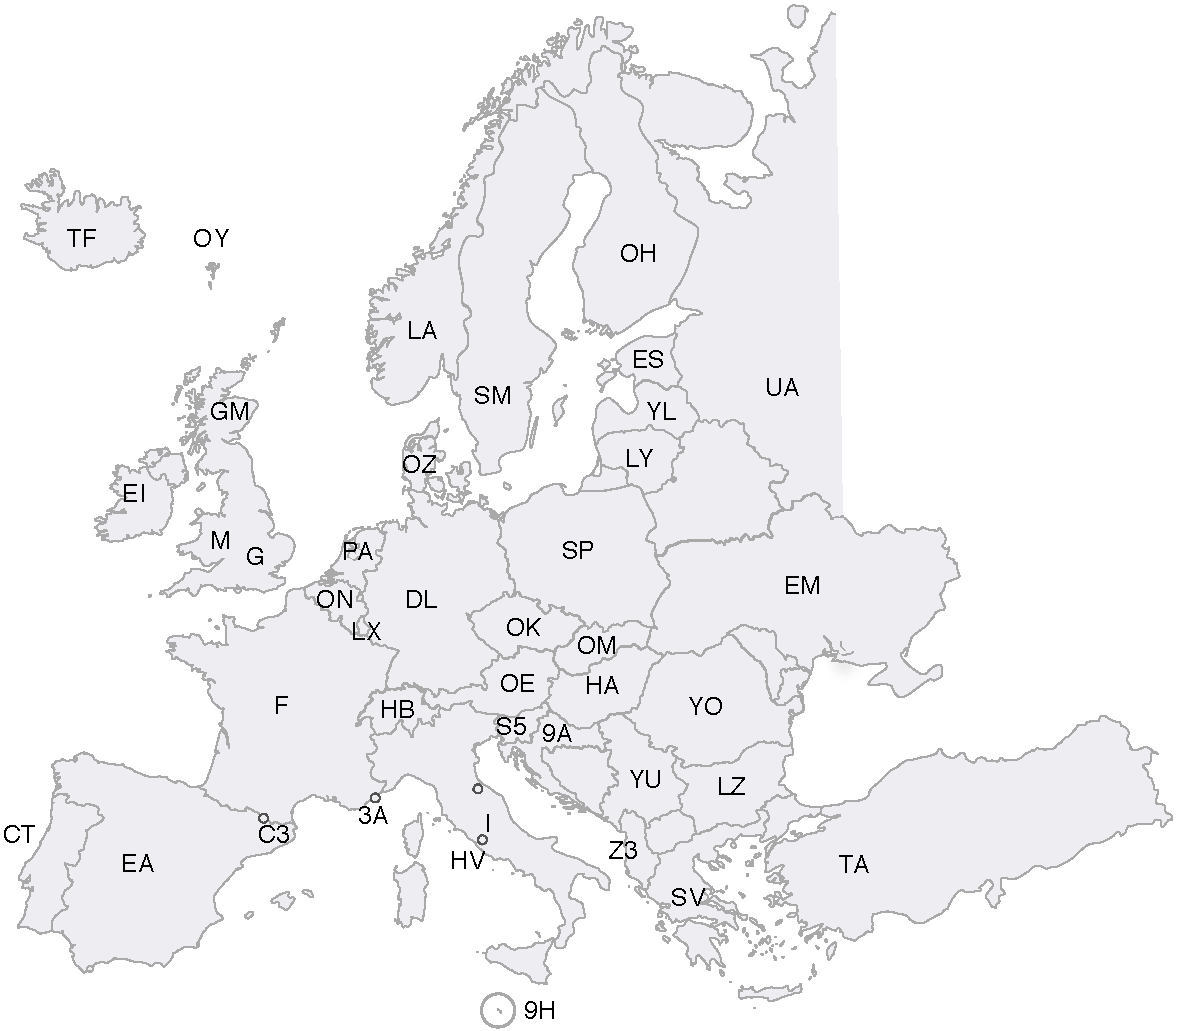
\includegraphics[width=14cm]{figures/landeskenner-eu}
	\label{fig:landeskenner-eu}
  \end{center}
\end{figure}


\subsection{Landeskenner Welt}\label{sec:landeskenner_welt}

Die Wellenausbreitung auf Mittelwelle lässt es zu, die Welt in drei
Regionen einzuteilen (RR):
\begin{enumerate}
  \item Region 1: Europa, Afrika, Vorderasien \& Russland
  \item Region 2: Nord- \& Südamerika, Karibik, Grönland, Hawaii
  \item Region 3: Australien, Neuseeland, Ozeanien \& das restliche
	Asien
\end{enumerate}

  \begin{longtable}{| l | l | l |}
  \hline
  Kenner & Land & Hint \\
  \hline
  \hline
  \endhead
  3V & Tunesien & \\
  \hline
  5N & Nigeria & \\
  \hline
  4X & Israel & \\
  \hline
  5B & Zypern & \\
  \hline
  5H & Tansania & \\
  \hline
  9X & Ruanda & \\
  \hline
  EL & Liberia & \\
  \hline
  ST & Sudan & \\
  \hline
  SU & Ägypten & \\
  \hline
  YK & Syrien & \\
  \hline
  ZS & Südafrika & \\
  \hline
\end{longtable}

\begin{figure}[htbp]
  \begin{center}
	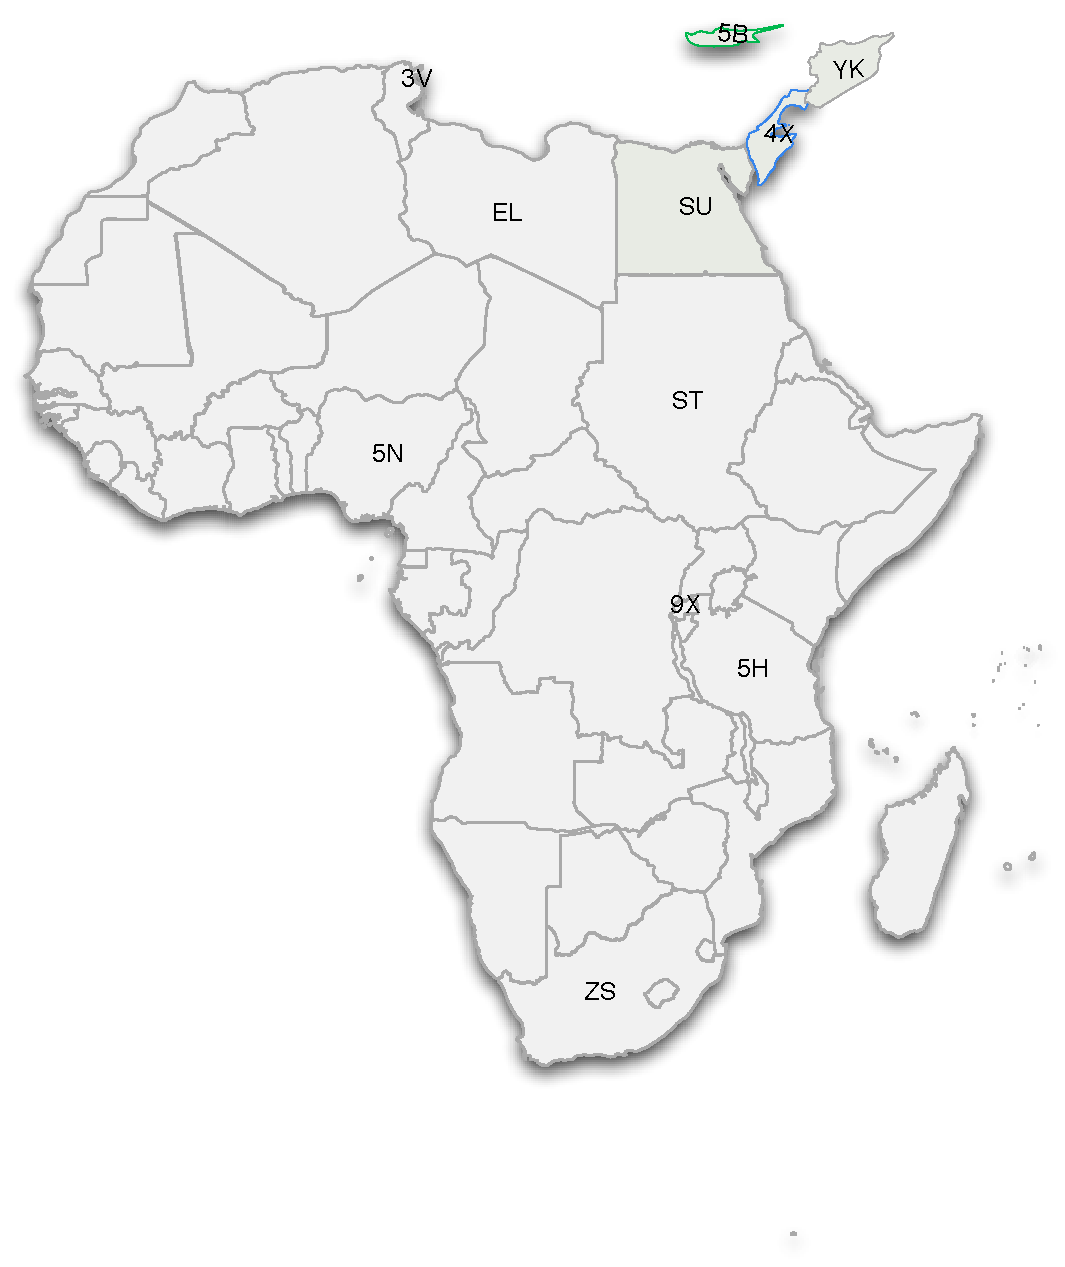
\includegraphics[width=14cm]{figures/landeskenner-afrika}
	\label{fig:landeskenner-afrika}
  \end{center}
\end{figure}

\begin{longtable}{| l | l | l |}
  \hline
  Kenner & Land & Hint \\
  \hline
  \hline
  \endhead
  \hline
  AA-AL, K, W, N & USA & \\
  \hline
  CE & Chile & \\
  \hline
  HC & Ecuador & \\
  \hline
  HK & Kolumbien & \\
  \hline
  LU & Argentinien & \\
  \hline
  OA & Peru & Obere Anden\\
  \hline
  PY & Brasilien & Pyranha\\
  \hline
  VE & Kanada & \\
  \hline
  XE, XF & Mexiko & \\
  \hline
  YV & Venezuela & \\
  \hline
\end{longtable}

\begin{figure}[h!]
  \begin{center}
	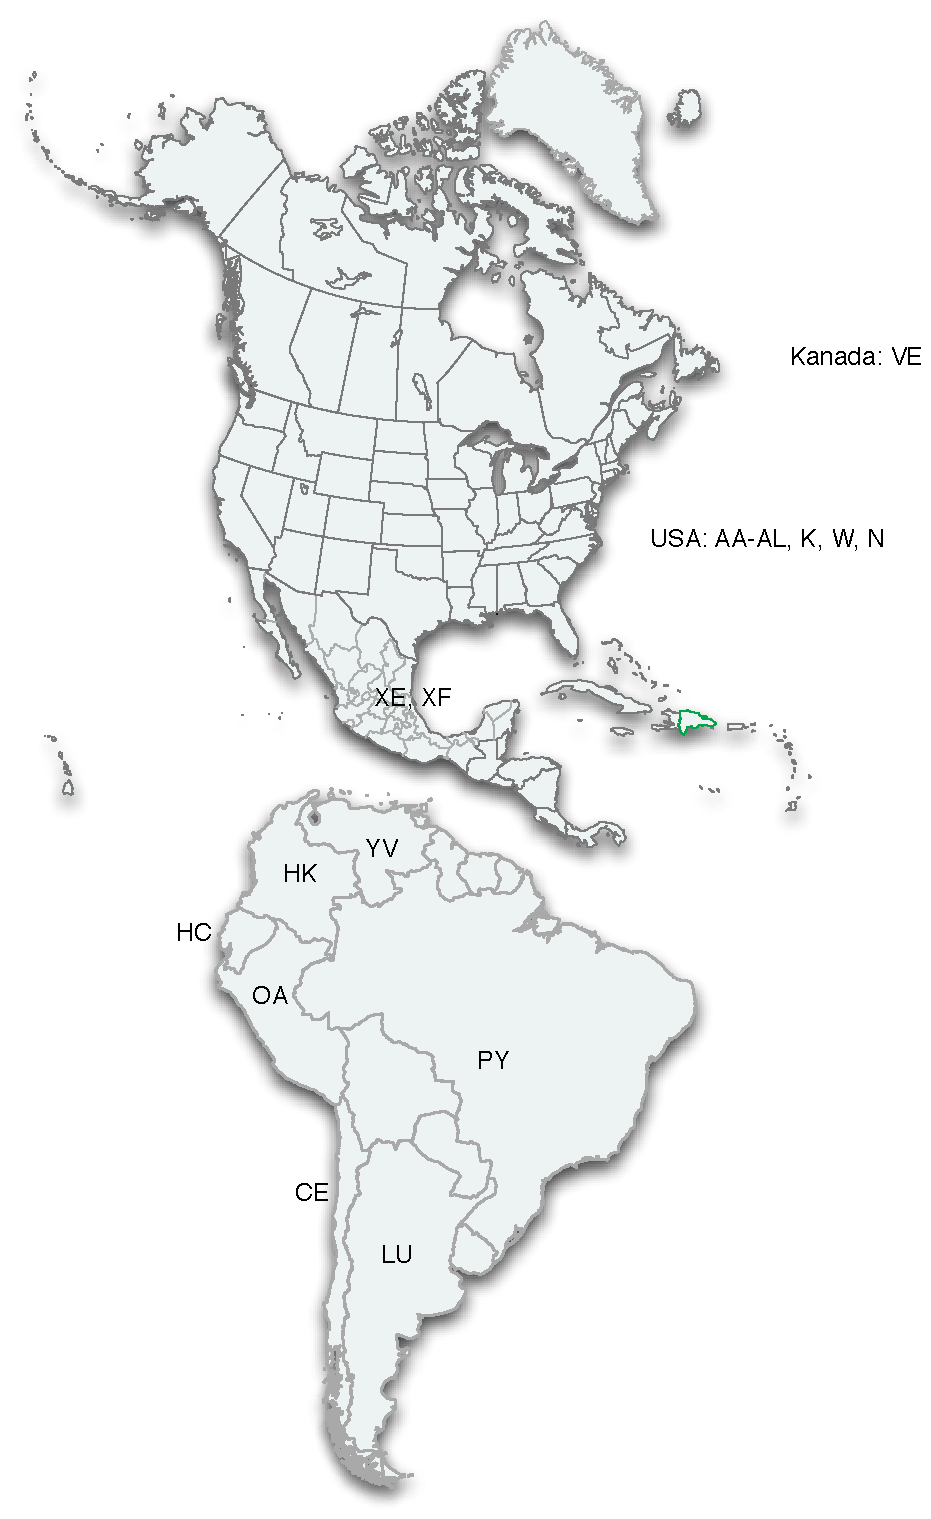
\includegraphics[width=14cm]{figures/landeskenner-amerika}
	\label{fig:landeskenner-amerika}
  \end{center}
\end{figure}

\begin{longtable}{| l | l | l |}
  \hline
  Kenner & Land & Hint \\
  \hline
  \hline
  \endhead
  4S & Sri Lanka & \\
  \hline
  BV & Taiwan & \\
  \hline
  BY & China & Billige Ypsgimmicks\\
  \hline
  DS-DT & Südkorea & \\
  \hline
  DU-DZ & Philippinen & \\
  \hline
  EP & Iran & \\
  \hline
  JA, JE-JS & Japan & \\
  \hline
  JT & Mongolei & \\
  \hline
  UA9, UA0 & Russland & \\
  \hline
  VK & Australien & Viele Känguruhs\\
  \hline
  VU & Indien & \\
  \hline
  ZL & Neuseeland & Zealand\\
  \hline
\end{longtable}



\begin{figure}[htbp]
  \begin{center}
	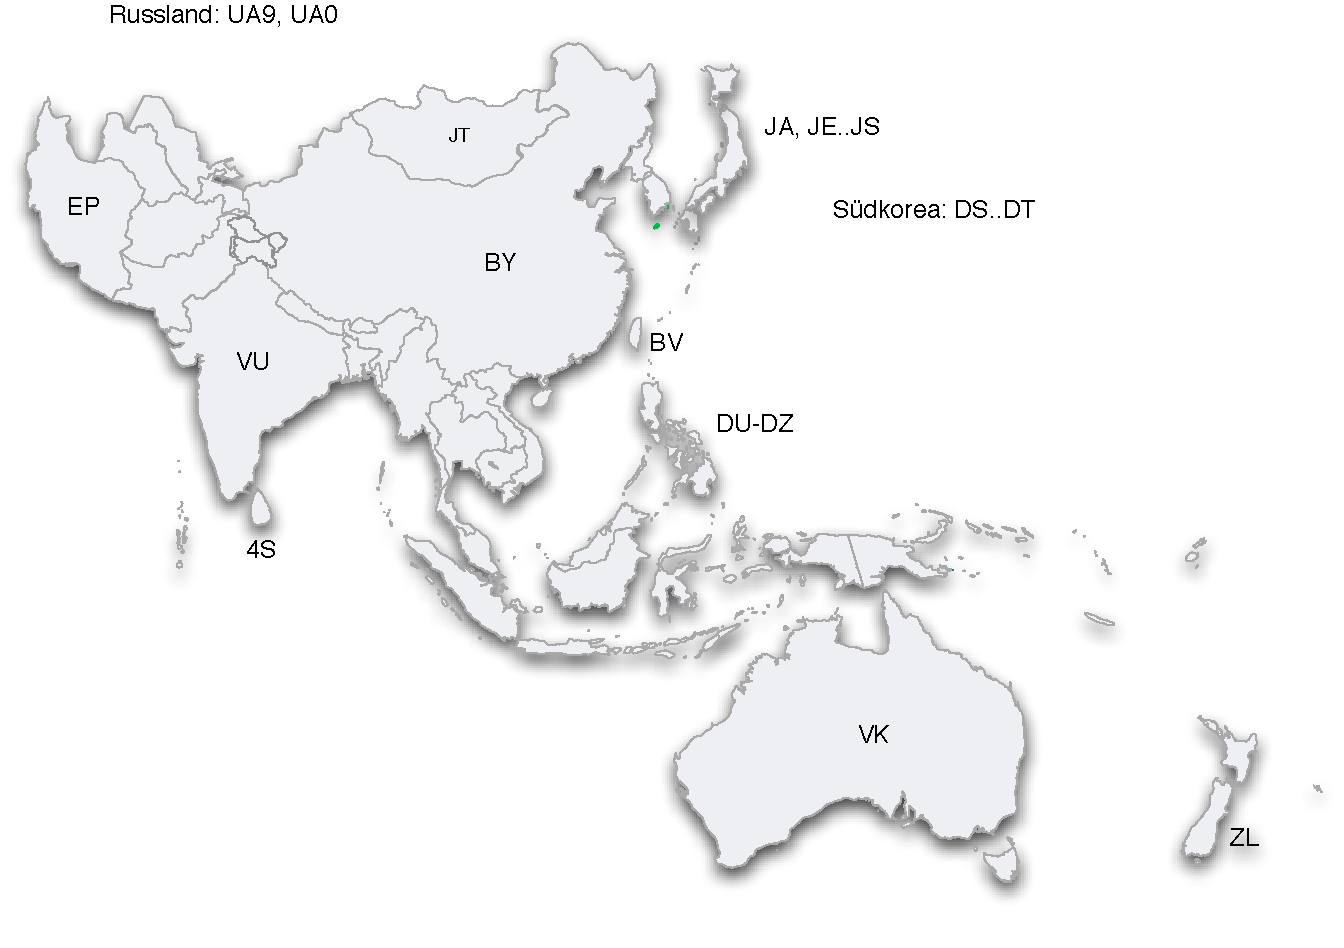
\includegraphics[width=14cm]{figures/landeskenner-region3}
	\label{fig:landeskenner-region3}
  \end{center}
\end{figure}


\subsection{Zusatzkennzeichen von Stationen}\label{sub:zusatzkennzeichen}
\begin{table}[h]
  \centering
\begin{tabular}{|l|l|}
  \hline
  /mm & Station auf offener See (marine mobile) \\
  /am & Station auf Luftfahrzeug (aeronautical mobile) \\
  /m & bewegliche Station auf anderem Fahrzeug (mobile) \\
  /p & Ortsfester Betrieb einer Station, optional (portabel) \\
  \hline
\end{tabular}
\end{table}

\subsection{Deutsche Rufkennzeichen}\label{sub:deutsche_rufkennzeichen}
Geregelt im Rufzeichenplan gem. §10(3) AFuV. In der Rufzeichenliste der
BNetzA sind alle zugeteilten Rufzeichen mit Name des Inhabers,
Relaisfunkstellen und Funkbaken registriert.

Deutsche Rufzeichen bestehen aus: 2 Buchstaben + Ziffer + 1-3
Buchstaben.

\begin{table}[h]
  \centering
\begin{tabular}{|l|l|}
  \hline
  DA..DM & Personengebundene Rufzeichen Klasse A\\
  \hline
  DO1..DO9 & Personengebundene Rufzeichen Klasse E\\
  \hline
  DF0, DG0, DH0, DK0, DL0, DM0 & Klubstationen Klasse A \\
  \hline
  DO0 & Klubstationen Klasse E \\
  \hline
  DN1..DN9 & Ausbildungsstation \\
  \hline
  DA0, DQ, DR & Kurzzeitstatio \\
  \hline
  DP0..DP1 & Exterritoriale Funkstelle \\
  \hline
  DA5U & Experimentelle Sonderstation \\
  \hline
  DB0 & Relaisfunkstelle, Digipeater, Funkbake\\
  \hline
\end{tabular}
\end{table}

\end{document}
